\chapter{\IfLanguageName{dutch}{Stand van zaken}{State of the art}}%
\label{ch:stand-van-zaken}

% Tip: Begin elk hoofdstuk met een paragraaf inleiding die beschrijft hoe
% dit hoofdstuk past binnen het geheel van de bachelorproef. Geef in het
% bijzonder aan wat de link is met het vorige en volgende hoofdstuk.

% Pas na deze inleidende paragraaf komt de eerste sectiehoofding.

% Dit hoofdstuk bevat je literatuurstudie. De inhoud gaat verder op de inleiding, maar zal het onderwerp van de bachelorproef *diepgaand* uitspitten. 
% De bedoeling is dat de lezer na lezing van dit hoofdstuk helemaal op de hoogte is van de huidige stand van zaken (state-of-the-art) in het onderzoeksdomein.
% Iemand die niet vertrouwd is met het onderwerp, weet nu voldoende om de rest van het verhaal te kunnen volgen, 
% zonder dat die er nog andere informatie moet over opzoeken \autocite{Pollefliet2011}.

% Je verwijst bij elke bewering die je doet, vakterm die je introduceert, enz.\ naar je bronnen. In \LaTeX{} kan dat met het commando \texttt{$\backslash${textcite\{\}}} of \texttt{$\backslash${autocite\{\}}}. Als argument van het commando geef je de ``sleutel'' van een ``record'' in een bibliografische databank in het Bib\LaTeX{}-formaat (een tekstbestand). Als je expliciet naar de auteur verwijst in de zin (narratieve referentie), gebruik je \texttt{$\backslash${}textcite\{\}}. Soms is de auteursnaam niet expliciet een onderdeel van de zin, dan gebruik je \texttt{$\backslash${}autocite\{\}} (referentie tussen haakjes). Dit gebruik je bv.~bij een citaat, of om in het bijschrift van een overgenomen afbeelding, broncode, tabel, enz. te verwijzen naar de bron. In de volgende paragraaf een voorbeeld van elk.

% \textcite{Knuth1998} schreef een van de standaardwerken over sorteer- en zoekalgoritmen. Experten zijn het erover eens dat cloud computing een interessante opportuniteit vormen, zowel voor gebruikers als voor dienstverleners op vlak van informatietechnologie~\autocite{Creeger2009}.

% Let er ook op: het \texttt{cite}-commando voor de punt, dus binnen de zin. Je verwijst meteen naar een bron in de eerste zin die erop gebaseerd is, dus niet pas op het einde van een paragraaf.

% \begin{figure}
%   \centering
%   \includegraphics[width=0.8\textwidth]{grail.jpg}
%   \caption[Voorbeeld figuur.]{\label{fig:grail}Voorbeeld van invoegen van een figuur. Zorg altijd voor een uitgebreid bijschrift dat de figuur volledig beschrijft zonder in de tekst te moeten gaan zoeken. Vergeet ook je bronvermelding niet!}
% \end{figure}

% \begin{listing}
%   \begin{minted}{python}
%     import pandas as pd
%     import seaborn as sns

%     penguins = sns.load_dataset('penguins')
%     sns.relplot(data=penguins, x="flipper_length_mm", y="bill_length_mm", hue="species")
%   \end{minted}
%   \caption[Voorbeeld codefragment]{Voorbeeld van het invoegen van een codefragment.}
% \end{listing}

% \lipsum[7-20]

% \begin{table}
%   \centering
%   \begin{tabular}{lcr}
%     \toprule
%     \textbf{Kolom 1} & \textbf{Kolom 2} & \textbf{Kolom 3} \\
%     $\alpha$         & $\beta$          & $\gamma$         \\
%     \midrule
%     A                & 10.230           & a                \\
%     B                & 45.678           & b                \\
%     C                & 99.987           & c                \\
%     \bottomrule
%   \end{tabular}
%   \caption[Voorbeeld tabel]{\label{tab:example}Voorbeeld van een tabel.}
% \end{table}
 
\section{PLC specificaties}
Volgende subcomponenten beschrijven wat een PLC is en hoe het opgezet is binnen het bedrijf.
Daarnaast wordt de manier van communicatie algemeen toegelicht en de dissectie van een bericht uiteengezet 
om inzicht te krijgen wat voor data er door het netwerk gaat.

\subsection{Wat is een PLC}
Een PLC (Programmable Logic Controller) is een industriële computer die wordt gebruikt voor het automatiseren van machines en processen \autocite{Bolton2015}. 
Het is ontworpen om robuust te zijn en betrouwbaar te functioneren in industriële omgevingen zoals in TVH, 
waar het wordt gebruikt om mechanische apparatuur, zoals transport systemen (conveyors) of liften van een automatisch magazijn te besturen.

\subsection{PLC gebruik binnen TVH}
Er zijn 7 verschillende PLC's in TVH Waregem die instaan voor verschillende zones van de conveyor.
Deze werden aangeleverd door Vanderlanden in het jaar 2013 en worden beheerd door het automatisatie team.
De communicatie tussen een PLC en het WCS is gebaseerd op het TCP/IP protocol en is verbonden via het intern netwerk.
Er is een tussenlaag tussen de PLC en het netwerk, RFC1006 van het merk Siemens waarin configuratie kan worden gedaan door het automatisatie team.
Dit stelt de collega's in staat om bepaalde logica te implementeren of netwerk aanpassingen door te voeren.
De snelheid van communicatie is essentieel, daarom moet het netwerk snel genoeg zijn zodat berichten aan een snel tempo verstuurd kunnen worden.

\subsection{PLC communicatie parameters}
De PLC's maken gebruik van een TCP/IP-socketverbinding en functioneren als client ten opzichte van het WCS, dat de rol van server vervult. 
Dit betekent dat de PLC de verbinding initieert en persisteert met de server die verantwoordelijk is voor de communicatie.
Een PLC is verantwoordelijk voor een specifieke zone van de conveyor en is opgebouwd uit drie kanalen die elk via een toegewezen poortnummer met de server communiceren. 
Meerdere kanalen zijn nodig om de communicatiesnelheid te bevorderen en omdat elk kanaal zijn eigen type informatie verwerkt~\autocite{Laar2013}.

\begin{table}
    \centering
    \begin{tabular}{lcr}
      \toprule
      \textbf{Kanaal} & \textbf{Beschrijving} & \textbf{Type}                \\
      \midrule
      1                & Route informatie over transportbak          & Snel           \\
      2                & Informatie van PLC                          & Niet kritisch  \\
      3                & Overige informatie over transportbak        & Snel           \\
      \bottomrule
    \end{tabular}
    \caption[Channel assignment]{\label{tab:channel-assignment}Beschrijving van kanalen}
  \end{table}

\subsection{PLC berichten}
Berichten bestaan uit een frame opgedeeld in velden en hebben een specifieke lengte.
De inhoud van een bericht is gebaseerd op het hexadecimale stelsel en wordt in detail toegelicht in de onderstaande tabel.
Bepaalde controles worden uitgevoerd om de validiteit van een bericht af te toetsen. 

\begin{table}[h!]
  \centering 
  \begin{tabular}{|c|c|c|c|}
    \hline
    \textbf{Veld} & \textbf{Inhoud} & \textbf{Data type} & \textbf{Lengte} \\
    % \hline
    % Dummy & Enkel PLC naar WCS
    \hline 
    Header & <STX> & Binair & 1 byte \\
    \hline 
    Lengte in bytes & 001D(HEX) & Binair & 2 bytes \\
    \hline 
    Seq. nummer &  [0-9] & ASCII & 1 byte  \\
    \hline 
    Inhoud & <...> & Binair & 27 bytes \\
    \hline 
    Terminator & <ETX> & Binair & 1 byte \\
    \hline
  \end{tabular}
  \caption[Message content]{\label{tab:message-content}Inhoud bericht}
\end{table}

Voorbeeld van een bericht dat van PLC naar WCS wordt verstuurd: 
\begin{listing}[h!]
  \begin{minted}{python}
    02 00 1d 20 30 36 20 20 00 00 20 20 30 37 20 20 30 20 20 20 20 20 20 20 20 20 20 20 20 20 20 03
  \end{minted}
  \caption[Voorbeeld PLC bericht]{Voorbeeld van een PLC bericht}
\end{listing}

Een bericht kan dus maximaal 32 bytes groot zijn en wordt in rekening gehouden voor de testen in latere fase.

\section{WCS specificaties}
In dit onderdeel wordt toegelicht wat een Warehouse Control System (WCS) is en welke verantwoordelijkheden dit systeem heeft.
Daarnaast wordt de structuur en werking van de communicatie tussen het systeem en de PLC uiteengezet.

\subsection{Wat is een WCS}
In het magazijn is de typische logistieke software het Warehouse Control System (WCS). 
Het WCS biedt een geïntegreerde interface voor een breed scala aan apparatuur. 
Het systeem kan de apparatuur in het magazijn beheren en aansturen~\autocite{Son2015}. 
 
\subsection{WCS communicatie} 
Binnen het bedrijf is het WCS een integraal deel uit van het monolithische ERP-pakket, waarvan TVH de eigenaar is van de code, geschreven in OpenEdge Progress 4GL. 
Het ERP-systeem draait op een server met acht verschillende batch-instanties die verantwoordelijk zijn voor de aansturing van de diverse PLC-kanalen. 
Elke batch-instantie communiceert met specifieke PLC-kanalen en bevat daarvoor specifieke logica.
Deze batches zijn verbonden via een specifieke poort met een Progress SonicMQ Adapter op de communicatie server.
Hiermee kunnen de batches de berichten consumeren en versturen van de SonicMQ server.

\subsection{WCS berichten} 
Berichten komen binnen van de PLC via de communicatie server. Ieder bericht wordt getransformeerd naar variabelen die dan verder gebruikt worden in de code.
Deze berichten bevatten informatie over transportbakken en zijn nodig om deze te kunnen traceren via de ERP.
Specifieke logica is nodig om bakken tot hun bestemming te krijgen, of om fout afhandeling te voorzien.
Volgende voorbeelden doen zich voor:
\begin{enumerate}
  \item Routeren naar een hospitaal punt door: 
  \begin{enumerate}
    \item Gewichtsfout
    \item Hoogtefout
    \item Onbekende bestemming
  \end{enumerate}
  \item Bestemming wordt gevraagd door de PLC
  \item Bestemming wordt doorgegeven aan de PLC 
  \item Specifieke logica moet uitgevoerd worden bij het passeren van een bepaald punt
  \item \dots
\end{enumerate}

\section{Communicatie tussen PLC en WMS}

De PLC kan alleen maar een TCP/IP socket verbinding initiëren met een server.
Omdat SonicMQ geen socket verbinding kan maken zijn er listeners gemaakt in Java door TVH.
Deze listeners fungeren als server en zijn specifiek opgesteld om een TCP/IP verbinding mogelijk te maken per PLC kanaal.
De Java listeners sturen de PLC-berichten vervolgens door naar SonicMQ of ontvangen berichten van SonicMQ, 
die ze via een socket naar de PLC doorsturen.
Aan de kant van het WCS zijn er meer mogelijkheden om verbinding te kunnen maken met een server.

De huidige opzet van het systeem kan je zien in onderstaande dataflow diagram:
\begin{figure}[h!]
  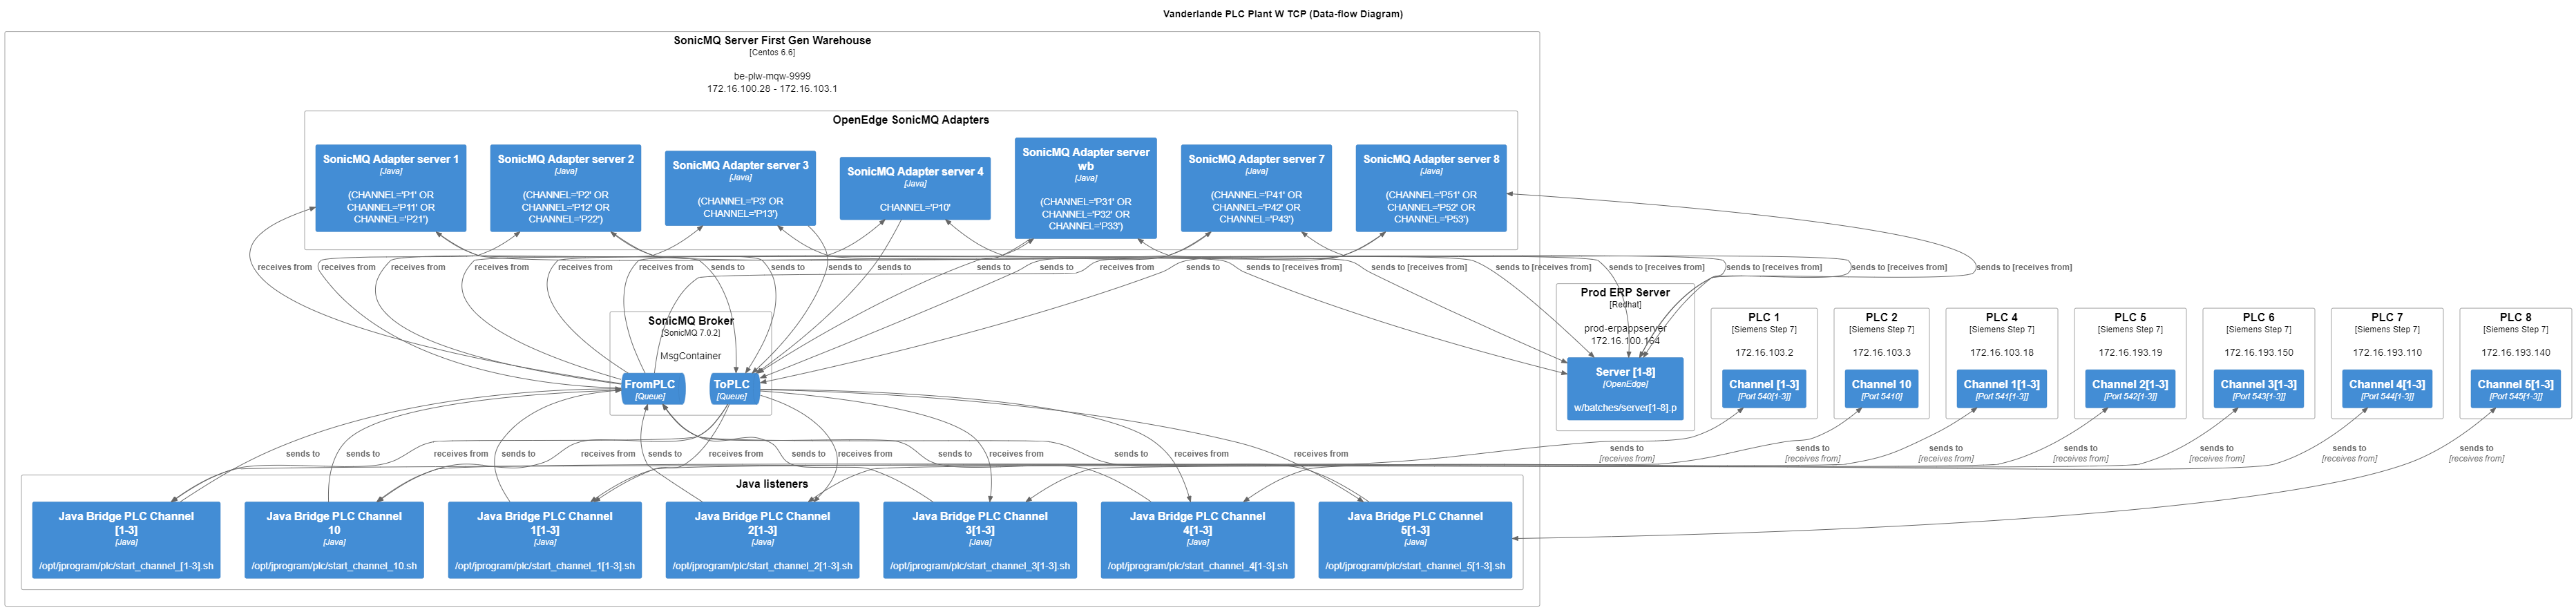
\includegraphics[width=0.9\textwidth]{img/plc-wcs_dataflow.png}
  \caption[Dataflow PLC]{\label{fig:dataflow-plc} Overzicht dataflow tussen PLC en WCS}
\end{figure}

\section{Soorten communicatie}
\emph{Inter-Process Communication (IPC)} omvat alle manieren van communicatie tussen services. 
Dit kan binnen hetzelfde systeem zijn of via een netwerk. 
Hieronder worden een aantal van deze communicatie methodes toegelicht.

\subsection{Shared memory}
Deze methode is relevant voor ons onderzoek omdat het gericht is op het delen van geheugenruimte 
tussen processen op hetzelfde systeem. 
Ze zijn nuttig voor het efficiënt delen van grote hoeveelheden data maar minder geschikt voor messaging, 
omdat ze geen ingebouwde mechanismen hebben voor het versturen van berichten ~\autocite{Dinari2020}.
 
\subsection{RPC-methoden voor messaging}
Hier worden de meest relevante \emph{Remote Procedure Call} (RPC) methoden besproken.

\subsubsection{XML en SOAP}
Deze methoden zijn relevant voor messaging omdat ze methoden en objecten via XML over HTTP kunnen aanroepen,
wat communicatie mogelijk maakt tussen verschillende platformen en programmeertalen.

\subsubsection{REST}
RESTful webservices gebruiken HTTP-verzoeken (zoals GET, POST) voor eenvoudige en efficiënte berichtuitwisseling, 
meestal in JSON formaat, wat ze zeer geschikt maakt voor messaging tussen webapplicaties.
Deze manier van communicatie is synchroon, waarbij de versturende partij moet wachten op antwoord.

\subsection{IPC-methoden voor Messaging}
Hier worden de meest relevante \emph{Inter Process Communication} (IPC) methoden besproken.

\subsubsection{Pipes}
\emph{Named pipes} hebben een synchrone werking en kunnen nuttig zijn, omdat ze bidirectionele 
communicatie tussen onafhankelijke processen mogelijk maken en kunnen functioneren tussen processen op hetzelfde systeem. \\
\emph{Ordinary pipes} bieden beperkte eenzijdige communicatie en vereisen een parent-child relatie, 
wat ze minder geschikt maakt voor messaging tussen onafhankelijke processen~\autocite{Dinari2020}.
 
\subsubsection{Socket}
Een socket-verbinding maakt gebruik van een endpoint gespecificeerd met een IP-adres en een poortnummer, 
waarmee twee autonome processen verbonden zijn, hetzij op dezelfde, hetzij op verschillende machines.
Streaming sockets (op basis van TCP) zijn nuttig voor betrouwbare, sequentiële berichtoverdracht, 
terwijl datagram sockets (op basis van UDP) geschikt zijn voor snelle, maar minder betrouwbare communicatie.
Beiden zijn synchroon en ondersteunen communicatie tussen verschillende netwerken en zijn veelgebruikt in messaging-applicaties~\autocite{Dinari2020}.
 
\subsubsection{Message queues} 
Messaging queues hebben een asynchrone werking, zijn \emph{socket-based} en maken gebruik van \emph{message queuing}, 
waarbij het de \emph{point-to-point} methodiek gebruikt.
Hierbij plaatst de \emph{producer} berichten in een specifieke queue, waarna een \emph{consumer} de berichten uitleest in een sequentiële volgorde.
Met andere woorden, een bericht wordt slechts aan één \emph{consumer} bezorgt.
\\
Dit maakt het voor applicaties mogelijk om asynchroon te communiceren zonder te moeten wachten op een antwoord van de ontvanger.
Ze zijn geschikt voor gedistribueerde systemen waar processen onafhankelijk werken~\autocite{Dinari2020}.

\subsubsection{Publish-Subscribe}
Het publish-subscribe-model is gebaseerd op topics waarop berichten worden gepubliceerd door de \emph{producer} 
en waar meerdere \emph{subscribers} (abonnees) zich kunnen op inschrijven. 
\\
In dit model ontvangen \emph{subscribers} slechts een subset van de totale gepubliceerde berichten. 
Het proces van het selecteren en verwerken van de berichten wordt filtering genoemd. 
Er zijn twee vormen van filtering: op basis van onderwerp (topic) en op basis van inhoud (content).
\\
In een op \emph{topic} gebaseerd systeem worden berichten geplaatst in \emph{topics} wat logische kanalen zijn.
\emph{Subscribers} ontvangen berichten van de \emph{topics} waarop ze zich hebben geabonneerd.
Alle \emph{subscribers} ontvangen dezelfde berichten uit dezelfde \emph{topics}. 
Deze methode zorgt voor een \emph{one-to-many} vorm van communicatie.
\\
Hierdoor ontvangen subscribers alleen de berichten uit de klassen die voor hen relevant zijn, zonder enige kennis van de publishers. 
Met het publish-subscribe-model specificeert de afzender nooit expliciet wie de ontvanger is en weet het zelfs niet of er al dan niet ontvangers zijn.

\begin{figure}[h!]
  \centering
  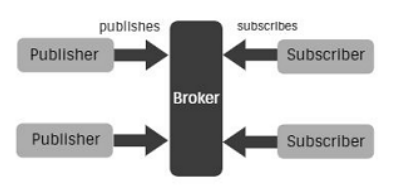
\includegraphics[width=.4\textwidth]{../voorstel/img/fig1-publish-subscribe.png}
  \caption{\label{fig:img}Publisher-Subscriber system\autocite{Sharvari2019}.}
\end{figure}


\subsection{Synchroon vs. asynchroon}
Services communiceren zowel \emph{synchroon} als \emph{asynchroon} en spelen deze benaderingen een cruciale rol, 
elk met hun eigen voor- en nadelen. \emph{Synchrone microservices} werken volgens een direct 
afhankelijkheidsmodel, omdat services met elkaar communiceren in een vraag-antwoordpatroon. 
Deze synchrone communicatie kan leiden tot ingewikkelde onderlinge afhankelijkheden, vertragingen en complexiteiten bij het debuggen 
van de logica. Bovendien wordt het schalen van synchrone services uitdagend, 
aangezien de schaalbaarheid van één service sterk afhankelijk is van andere services die het gebruikt \autocite{Bellemare2020}. 
Deze manier van communicatie kan niet voldoen aan de niet-functionele eisen van het automatisch magazijn binnen TVH.
\newline

Daartegenover heeft \emph{asynchrone} communicatie een reeks voordelen. Ze bieden grotere schaalbaarheid, technologische 
flexibiliteit en aanpassingsvermogen aan veranderende zakelijke vereisten. 
In plaats van de synchrone manier van communicatie is de \emph{asynchrone} gemakkelijker te herstructureren en te onderhouden. 
Ze vergemakkelijken \emph{continuous delivery} door hun onafhankelijkheid omdat de communicatie 
met een \emph{messaging systeem} opgevangen wordt. 
Hun verminderde afhankelijkheden en geïsoleerde karakter maken het testen relatief eenvoudiger en robuuster.
Het enige grote nadeel in asynchrone communicatie is \emph{error handling}, 
omdat dit niet opgevangen kan worden door de verzendende partij.
\newline

\begin{figure}[h!]
  \centering
  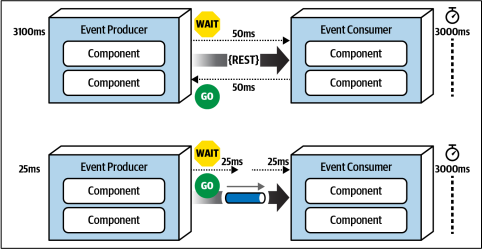
\includegraphics[width=.5\textwidth]{../voorstel/img/synchronous_vs_async_calls.png}
  \caption{\label{fig:img}Synchronous versus asynchronous communication \autocite[figure 14 -- 13]{MarkRichards2021}.}
\end{figure}

In praktische termen is het vinden van de juiste balans tussen synchrone en \emph{asynchrone microservices} cruciaal, 
afhankelijk van de specifieke behoeften van een organisatie en de aard van haar bedrijfsprocessen. 
Een hybride aanpak waarin beide architecturen naast elkaar bestaan en elkaar aanvullen blijkt vaak de meest effectieve strategie te zijn. 
Deze aanpak stelt organisaties in staat om de sterke punten van zowel synchrone als asynchrone modellen te benutten, 
waardoor flexibiliteit, schaalbaarheid en onderhoudsgemak worden gegarandeerd in complexe \newline IT-landschappen.
In deze paper ligt de focus op \emph{asynchrone communicatie} voor het gebruik van \emph{messaging systemen}.
\newline
 

\section{Wat is een EoL systeem}

\section{Wat zijn de gevaren van EoL systemen}

\section{Welke manieren zijn er om EoL weg te werken}


